\documentclass[11pt,letterpaper]{article}
\usepackage[lmargin=1in,rmargin=1in,tmargin=1in,bmargin=1in]{geometry}
\usepackage{../style/homework}
\usepackage{../style/commands}
\setbool{quotetype}{true} % True: Side; False: Under
\setbool{hideans}{true} % Student: True; Instructor: False

% -------------------
% Content
% -------------------
\begin{document}

\homework{10: Due 06/14}{Somewhere, something incredible is waiting to be known.}{Carl Sagan}

% Problem 1
\problem{10} Sketch the function $f(x)= \dfrac{11}{3} \left( \dfrac{1}{2} \right)^x$ as accurately as possible on the graph below. 
	\[
	\fbox{
	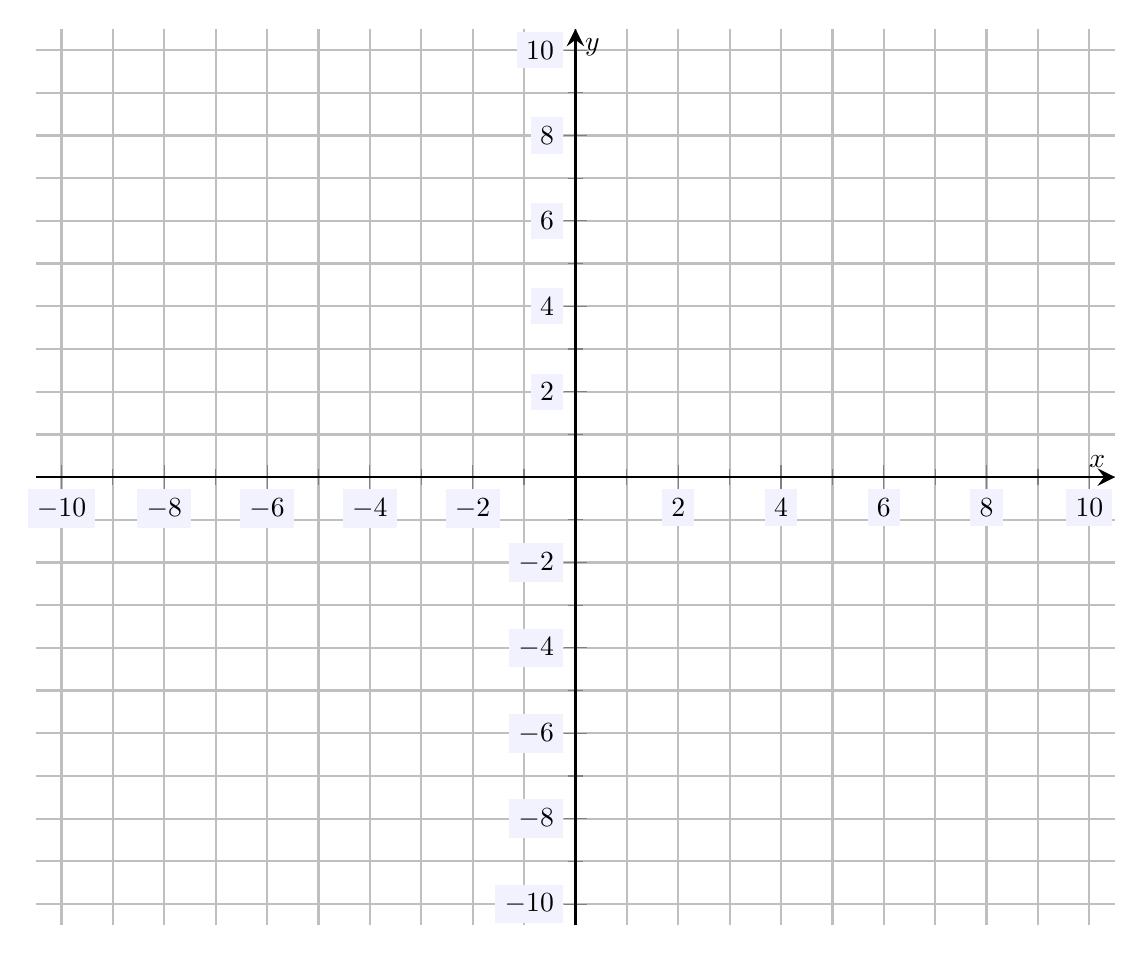
\begin{tikzpicture}[scale=2,every node/.style={scale=0.5}]
	\begin{axis}[
	grid=both,
	axis lines=middle,
	ticklabel style={fill=blue!5!white},
	xmin= -10.5, xmax=10.5,
	ymin= -10.5, ymax=10.5,
	xtick={-10,-8,-6,-4,-2,0,2,4,6,8,10},
	ytick={-10,-8,-6,-4,-2,0,2,4,6,8,10},
	minor tick = {-10,-9,...,10},
	xlabel=\(x\),ylabel=\(y\),
	]
	\end{axis}
	\end{tikzpicture}
	}
	\] 



\newpage



% Problem 2
\problem{10} Showing all your work, determine whether the following functions are increasing or decreasing:
	\begin{enumerate}[(a)]
	\item $-5 \left( 2 \right)^{-\frac{1}{5} x}$
	\item $\dfrac{7}{8} \left( \dfrac{5}{6} \right)^{4x}$
	\item $17 \left( \dfrac{5}{4} \right)^{-x}$
	\item $-10 \left( \dfrac{1}{3} \right)^{-5x}$
	\end{enumerate}



\newpage



% Problem 3
\problem{10} Showing all your work, solve the following equation:
	\[
	2^{3x}= 4
	\]



\newpage



% Problem 4
\problem{10} Showing all your work, solve the following equation:
	\[
	7(4^{1 - x})= \dfrac{7}{16}
	\]



\newpage



% Problem 5
\problem{10} Showing all your work, solve the following equation:
	\[
	\dfrac{1}{3^x}= 27^{\frac{4x + 10}{3}}
	\]



\newpage



% Problem 6
\problem{10} Showing all your work, solve the following equation:
	\[
	5^{x - 2} + 6= 11
	\]



\newpage



% Problem 7
\problem{10} Showing all your work, solve the following equation:
	\[
	\dfrac{1}{4^x}= 1024
	\]



\newpage



% Problem 8
\problem{10} Showing all your work, solve the following equation:
	\[
	\left( \dfrac{2}{3} \right)^{5x - 7}= 1
	\]



\newpage



% Problem 9
\problem{10} Suppose you invest \$5,000 in an account which earns 4.6\% annual interest, compounded quarterly. How much will be in the account after 3~years?



\newpage


% Problem 10
\problem{10} If you take out a loan for \$1,200 at a 5.5\% annual interest, compounded continuously, how much is owed after 2~years? How much of this amount is interest?


\end{document}